%%%%%%%%%%%%%%%%%%%%%%%%%%%%%%%%%%%%%%%%%%%%%%%%%%%%%%%%%%%%%%%%%%%%%
% PREAMBLE
%%%%%%%%%%%%%%%%%%%%%%%%%%%%%%%%%%%%%%%%%%%%%%%%%%%%%%%%%%%%%%%%%%%%%
%
% The following two commands will generate a PDF that follows all the requirements for submission
% and peer review.  Uncomment these commands to generate this output (and comment out the two lines below.)
%
% DOUBLE SPACE VERSION FOR SUBMISSION TO THE AMS
\documentclass[12pt]{article}
\usepackage{ametsoc}
%
% The following two commands will generate a single space, double column paper that closely
% matches an AMS journal page.  Uncomment these commands to generate this output (and comment
% out the two lines above. FOR AUTHOR USE ONLY. PAPERS SUBMITTED IN THIS FORMAT WILL BE RETURNED
% TO THE AUTHOR for submission with the correct formatting.
%
% TWO COLUMN JOURNAL PAGE LAYOUT FOR AUTHOR USE ONLY
%%%%\documentclass[10pt]{article}
%%%%\usepackage{ametsoc2col}
%
%%%%%%%%%%%%%%%%%%%%%%%%%%%%%%%%%%%%%%%%%%%%%%%%%%%%%%%%%%%%%%%%%%%%%
% ABSTRACT
%
% Enter your Abstract here
%%%%%%%%%%%%%%%%%%%%%%%%%%%%%%%%%%%%%%%%%%%%%%%%%%%%%%%%%%%%%%%%%%%%%
\newcommand{\myabstract}{Enter abstract here.}
%
\begin{document}
%
%%%%%%%%%%%%%%%%%%%%%%%%%%%%%%%%%%%%%%%%%%%%%%%%%%%%%%%%%%%%%%%%%%%%%
% TITLE
%
% Enter your TITLE here
%%%%%%%%%%%%%%%%%%%%%%%%%%%%%%%%%%%%%%%%%%%%%%%%%%%%%%%%%%%%%%%%%%%%%
\title{\textbf{\large{A Sample American Meteorological Society \LaTeX\ Document}}}
%
% Author names, with corresponding author information. 
% [Update and move the \thanks{...} block as appropriate.]
%
\author{\textsc{Brian Papa}
				\thanks{\textit{Corresponding author address:} 
				Brian Papa, American Meteorological Society, 
				45 Beacon St., Boston, MA 01464. 
				\newline{E-mail: latex@ametsoc.org}}\quad\textsc{and Sarah Cooley}\\
\textit{\footnotesize{American Meteorological Society, Boston, Massachusetts}}
\and 
\centerline{\textsc{Extra Author}}\\% Add additional authors, different insitution
\centerline{\textit{\footnotesize{Affiliation, City, State/Province, Country}}}
}
%
% Formatting done here...Authors should skip over this.  See above for abstract.
\ifthenelse{\boolean{dc}}
{
\twocolumn[
\begin{@twocolumnfalse}
\amstitle

% Start Abstract (Enter your Abstract above.  Do not enter any text here)
\begin{center}
\begin{minipage}{13.0cm}
\begin{abstract}
	\myabstract
	\newline
	\begin{center}
		\rule{38mm}{0.2mm}
	\end{center}
\end{abstract}
\end{minipage}
\end{center}
\end{@twocolumnfalse}
]
}
{
\amstitle
\begin{abstract}
\myabstract
\end{abstract}
}
%%%%%%%%%%%%%%%%%%%%%%%%%%%%%%%%%%%%%%%%%%%%%%%%%%%%%%%%%%%%%%%%%%%%%
% MAIN BODY OF PAPER
%%%%%%%%%%%%%%%%%%%%%%%%%%%%%%%%%%%%%%%%%%%%%%%%%%%%%%%%%%%%%%%%%%%%%
\section{First primary heading}

\section{Second primary heading}

\subsection{First secondary heading}

\subsection{Second secondary heading}

\subsubsection{First tertiary heading}

\subsubsection{Second tertiary heading}

\paragraph{First quaternary heading}

\paragraph{Second quaternary heading}

\section{Third primary heading}

\subsection*{First unnumbered secondary heading}

\subsubsection*{First unnumbered tertiary heading}

\paragraph*{First unnumbered quaternary heading}

\section{Fourth primary heading}

\begin{acknowledgment} 
Start acknowledgments here.
\end{acknowledgment}

% Use appendix}[A], {appendix}[B], etc. etc. in place of appendix if you have multiple appendixes.
\ifthenelse{\boolean{dc}}
{}
{\clearpage}
\begin{appendix}
\section*{\begin{center}Appendix Title Is Entered Here (Primary heading)\end{center}}
\subsection{First appendix secondary heading}

\subsection{Second appendix secondary heading}

\subsubsection{First appendix tertiary heading}

\subsubsection{Second appendix tertiary heading}

\paragraph{First appendix quaternary heading}

\paragraph{Second appendix quaternary heading}

\end{appendix}

% Create a bibliography directory and place your .bib file there.
\ifthenelse{\boolean{dc}}
{}
{\clearpage}
\bibliographystyle{./ametsoc}
\bibliography{./bibliography/references}

%%%%%%%%%%%%%%%%%%%%%%%%%%%%%%%%%%%%%%%%%%%%%%%%%%%%%%%%%%%%%%%%%%%%%
% FIGURES
%%%%%%%%%%%%%%%%%%%%%%%%%%%%%%%%%%%%%%%%%%%%%%%%%%%%%%%%%%%%%%%%%%%%%
\begin{figure}[t]
  \noindent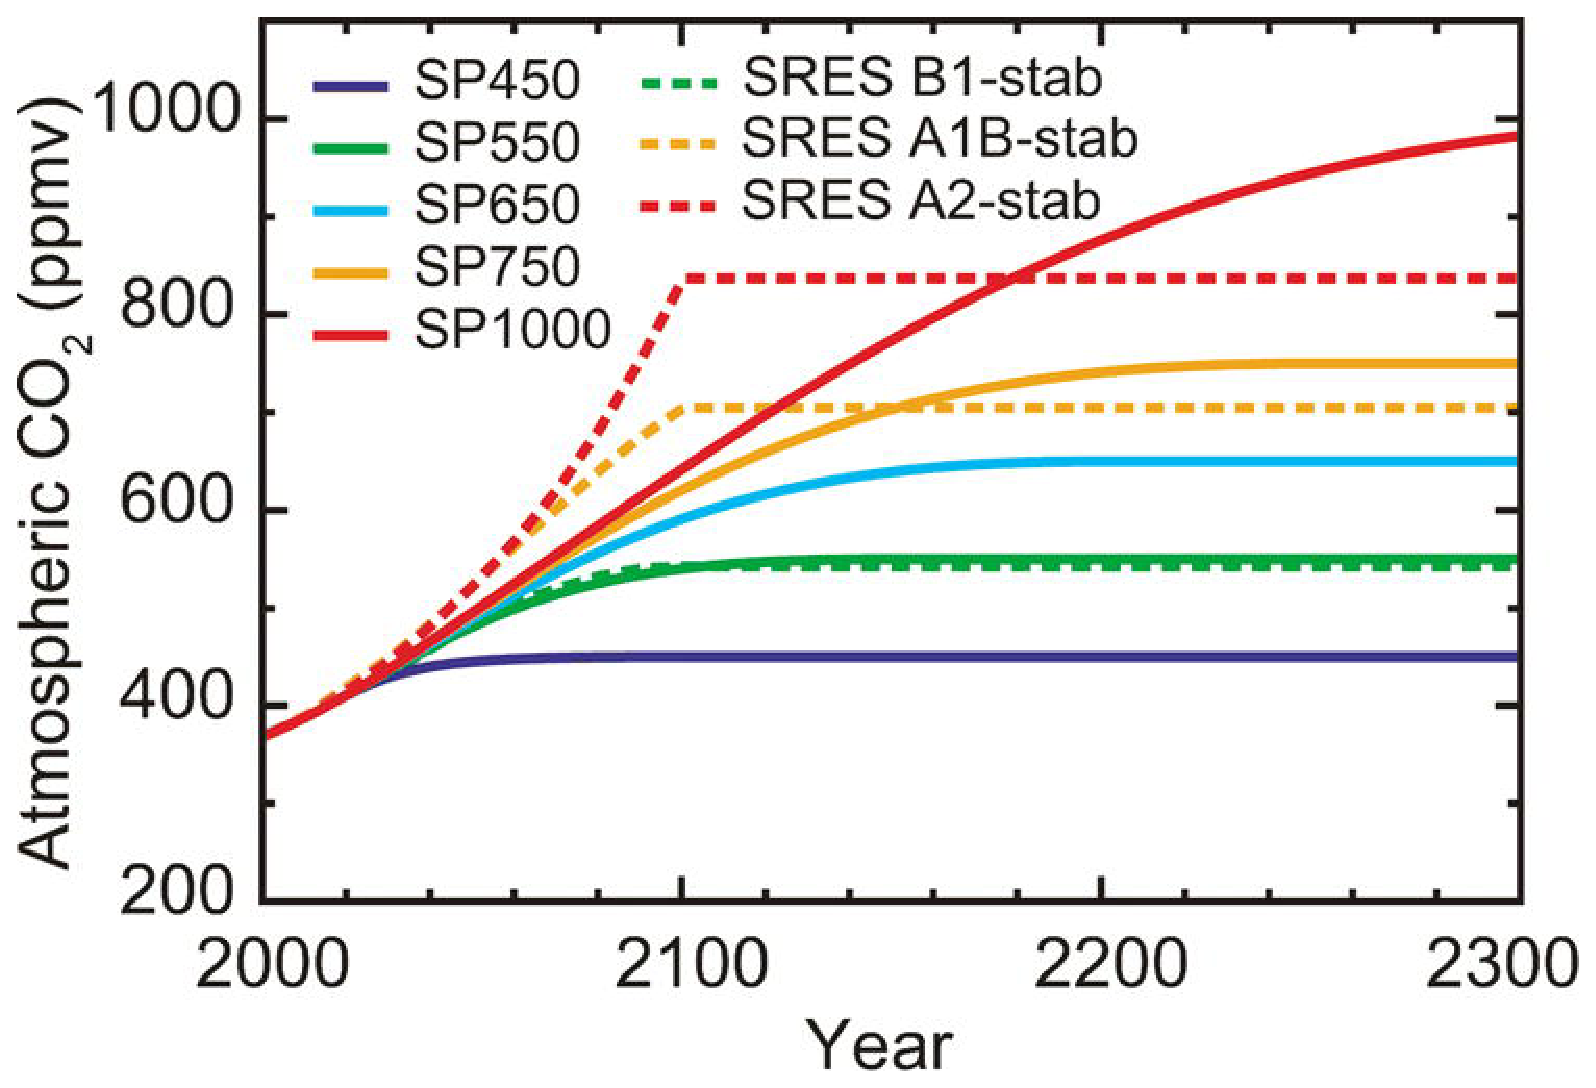
\includegraphics[width=19pc,angle=0]{./figures/figure01.eps}\\
  \caption{Enter the caption for your figure here.  Repeat as
  necessary for each of your figures. Create a figures directory and
  place all figures in that directory. Figure from Houghton et al. (2001).}\label{f1}
\end{figure}
%%%%%%%%%%%%%%%%%%%%%%%%%%%%%%%%%%%%%%%%%%%%%%%%%%%%%%%%%%%%%%%%%%%%%
% TABLES
%%%%%%%%%%%%%%%%%%%%%%%%%%%%%%%%%%%%%%%%%%%%%%%%%%%%%%%%%%%%%%%%%%%%%
\begin{table}[t]
\caption{This is a sample table caption and table layout.  Enter as many tables as
  necessary at the end of your manuscript. Table from Lorenz (1963).}\label{t1}
\begin{center}
\begin{tabular}{ccccrrcrc}
\hline\hline
$N$ & $X$ & $Y$ & $Z$\\
\hline
 0000 & 0000 & 0010 & 0000 \\
 0005 & 0004 & 0012 & 0000 \\
 0010 & 0009 & 0020 & 0000 \\
 0015 & 0016 & 0036 & 0002 \\
 0020 & 0030 & 0066 & 0007 \\
 0025 & 0054 & 0115 & 0024 \\
\hline
\end{tabular}
\end{center}
\end{table}
%
\end{document}